\documentclass[a4paper]{article}
%% Welcome to Overleaf!
%% If this is your first time using LaTeX, it might be worth going through this brief presentation:
%% https://www.overleaf.com/latex/learn/free-online-introduction-to-latex-part-1

%% Researchers have been using LaTeX for decades to typeset their papers, producing beautiful, crisp documents in the process. By learning LaTeX, you are effectively following in their footsteps, and learning a highly valuable skill!

%% The \usepackage commands below can be thought of as analogous to importing libraries into Python, for instance. We've pre-formatted this for you, so you can skip right ahead to the title below.

%% Language and font encodings
\usepackage[spanish,english]{babel}
\usepackage[utf8x]{inputenc}
\usepackage[T1]{fontenc}

%% Sets page size and margins
\usepackage[a4paper,top=2cm,bottom=2cm,left=3cm,right=3cm,marginparwidth=1.75cm]{geometry}

%% Useful packages
\usepackage{amsmath}
\usepackage{graphicx}
\usepackage[colorinlistoftodos]{todonotes}
\usepackage[colorlinks=true, allcolors=blue]{hyperref}
\usepackage{float}

%% Title
\title{
		%\vspace{-1in} 	
		\usefont{OT1}{bch}{b}{n}
		\normalfont \normalsize \textsc{CSE-4111 Artificial Intelligence Lab} \\ [10pt]
		\huge Final Assignment : Name Nationality Classification with Recurrent Neural Networks \\
}

\usepackage{authblk}
\author[0]{\textbf{Saif Mahmud}\\
		4th Year 1st Semester, Roll : SH - 054\\}


\begin{document}
\maketitle

\selectlanguage{english}
\begin{abstract}
This assignment involves the task of classification of nomenclature text data into their respective nationality or ethnicity. Recurrent Neural Network (RNN) has been used in the regard of accomplishing this task. In order to build the neural network model, I have followed the model architecture described in \cite{lee2017name}. The paper has described the model with RNN variant Long Short Term Memory (LSTM) in order to overcome the bottlenecks on long-term dependency and I have built the model accordingly with the particular embedding technique specified by the authors.  
\end{abstract}

\section*{Problem Formulation}
The problem of this assignment is defined as the task of predicting nationality or ethnicity given the personal name. In order to feed the sequential input to the neural network, the model incorporates LSTM architecture. However, the dataset for this model is a simple one with name as input feature and country as class label. Here, the input feature is sequential data of character embedding which refers to the fixed-size vector representation of specific character set. On the other hand, the class label is indexed alphabetically for the multi-class classification task and it is accomplished with softmax unit in accordance with the model description of \cite{lee2017name}. 


\section*{Model Architecture}
Recurrent Neural Networks (RNNs) play an efficient role in case of sequence modeling and here personal name is considered as sequence of input data. Nevertheless, conventional RNNs suffer form long-term dependency problem and as a result Long Short Term Memory (LSTM) emerges as the recurrent unit taken into consideration in building of name nationality classification task.
\\

In order to feed the LSTM units with fixed-size representation of vector, an embedding architecture is constructed. However, the authors of \cite{lee2017name} has proposed character-level embedding with n-gram. Here, n-gram refers to contiguous sequence of n items from the given text data and I have taken the case of unigram, bigram and trigram into account. Therefore, the input training data is segmented into n-grams and trained with a word2vec model with skip-gram into a vector representation of size 100. It should be noted that I have assumed the use of skip-gram window of size 5 as an empirical value which is not mentioned in the paper \cite{lee2017name} and trained the character level embedding model with the library `gensim'. This pre-trained embedding model will be used later for obtaining 100 size vector representation of particular n-gram word set.
\\

LSTM incorporates a memory cell and forget gate along with the conventional hidden state of RNNs and this forget gate enables LSTM to capture long-term dependency and produce particular input specific context vector for classification task. In the procedure of construction of LSTM with Keras with Tensorflow back-end, the first layer is specified as embedding layer. The embedding layer is supplied with the one hot representation of input n-gram character set and here the one-hot vector representation is defined as a sparse vector with index entry of n-gram character set as 1 and the rest as 0. However, this one-hot vector is multiplied with the pre-trained embedding vector to fetch the specific fixed-size representation for n-gram character set.
\\

In the implementation of second layer, the LSTM is created with specified dropout of 0.5 in accordance with the paper \cite{lee2017name}. Here, dropout is taken as the technique of regularization to cope with overfitting problem. The idea of dropout refers to dropping random units in the neural network architecture to provide generalization in training and the value indicates how much fraction of neurons to be dropped randomly.
\\

The loss function for LSTM model is defined as cross-entropy loss function and the model is trained through backpropagation with learning rate of 0.0035. Here, I did not tune the hyperparameters on validation set, rather used the specified ones in \cite{lee2017name}. The optimization algorithm defined for this LSTM architecture is `adam' and the model was trained on input data for 15 epochs. The authors evaluated the performance on the metric accuracy and I have incorporated the same as evaluation metric. As this is a multi-class classification problem, so precision-recall or $ F_{1} $-score will not serve the purpose. Therefore, I have created a confusion matrix on a subset of test examples to illustrate the misclassifications in visualization and Area Under Curve (AUC) ,which is a good metric in imbalanced class scenario, can be calculated from the confusion matrix entries.

\begin{figure}[ht!]
	\centering
	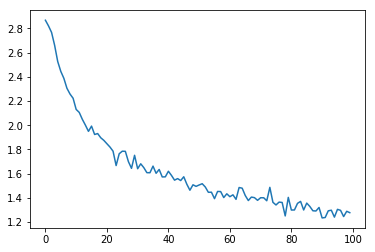
\includegraphics[width = 0.5\columnwidth, height = 5.5cm]{loss.png}
	\caption{Value of Loss Function During Training of LSTM}
	\label{fig:loss}
\end{figure}

In Figure \ref{fig:loss}, the value of loss function is plotted and is an indication that the model converges to global optima through backpropagation in the case of LSTM embodied with bigram embedding on character vector. 

\section*{Result and Discussion}
t-Distributed Stochastic Neighbor Embedding (t-SNE) is a technique for dimensionality reduction that is particularly well suited for the visualization of high-dimensional datasets. In the paper \cite{lee2017name} in our consideration, the authors has visualized the unigram and bigram embedding of vector size 100 with t-SNE. Here, in this experiment I have reduced the dimensionality for trigram embedding vector of size 100 into 2D through t-SNE transformation with `Scikit-learn' library and visualized this with `matplotlib' which is given below: 
\\

\begin{figure}[t!]
	\centering
	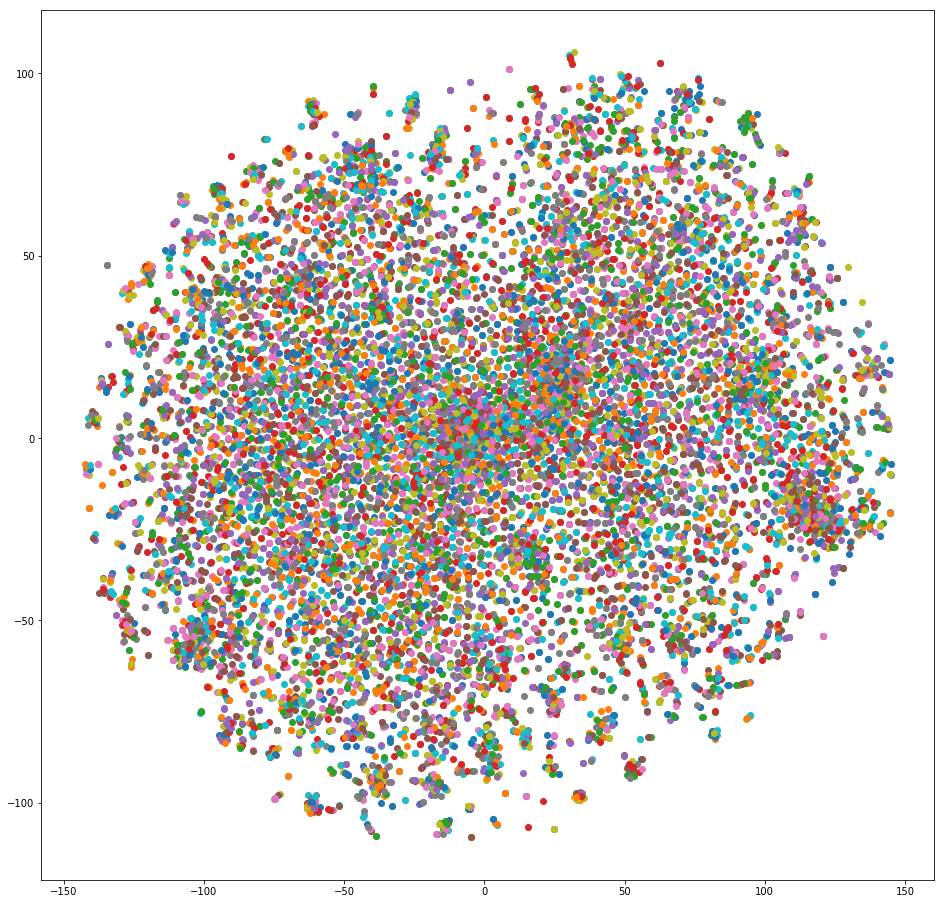
\includegraphics[width = 0.95\columnwidth, height = 13cm]{tsne.png}
	\caption{t-SNE of Trigram Embedding Vector}
	\label{fig:tsne}
\end{figure}

In Figure \ref{fig:tsne}, the visualization of trigram embedding vector is illustrated and it indicates that points in vicinity has more syntactic and semantic similarity.
\\

The accuracy of proposed model architecture is determined by the ratio of correct class labeling with the learned parameters and total number of records for classification in the training data. The mathematical expression of accuracy provided in \ref{eqn:accuracy} where TP, TN, FP and FN is defined as True Positive, True Negative, False Positive and False Negative respectively.

\begin{equation}
\label{eqn:accuracy}
Accuracy = \frac{TP + TN}{TP + TN + FP + FN}
\end{equation}

\begin{table}[t!]
	\centering
	\caption{Accuracy of Implemented LSTM Model Architecture}
	\label{table:acc}
	\begin{tabular}{|c|c|}
		\hline
		\textbf{Model Architecture} & \textbf{Accuracy (\%)} \\ \hline
		LSTM + Unigram (Embedding)  & 84.06                   \\ \hline
		LSTM + Bigram (Embedding)   & 84.84                  \\ \hline
		LSTM + Trigram (Embedding)  & 80.64                  \\ \hline
	\end{tabular}
\end{table}

In Table \ref{table:acc}, the accuracy of LSTM model along with n-gram character level embedding vector on predefined test examples are shown.

Confusion matrix is defined as a measurement on machine learning algorithms to evaluate the performance of classification task in multi-class scenario. I have selected a subset of ethnicity and visualized the confusion matrix to demonstrate the correct and wrong class labeling characteristics.
\\

\begin{figure}[t!]
	\centering
	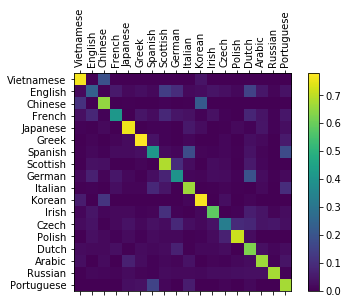
\includegraphics[width = 0.5\columnwidth, height = 6.5cm]{confusion.png}
	\caption{Confusion Matrix}
	\label{fig:conf_mat}
\end{figure}

In Figure \ref{fig:conf_mat}, the diagonal entries in the matrix indicates correct class label with are the brightest ones due to the model's high accuracy. On the other hand, the mislabeled entries demonstrates which of the classes are acute in creating confusion in class labeling for a particular class due to very close decision boundary.

\section*{Conclusion}
To reverse engineer a particular paper, is a challenging task to accomplish because I had to make certain assumptions on the implementation which is not described in the manuscript explicitly. Nevertheless, despite building an RNN model (LSTM) on sequential data for personal name classification based on country or ethnicity has some performance tuning issue and data preprocessing issue including the construction of embedding vector in character level, it was accomplished with a high accuracy in specified task.

\bibliography{refs} 
\bibliographystyle{ieeetr}

\end{document}
